% ============================================================
%  eMeter AMU — Comprehensive Actor & Module Documentation
%  Aligarh Muslim University Electricity Management System
%  Author: Project Documentation
%  Date:   2026
% ============================================================

\documentclass[12pt, a4paper]{report}

% ─── Packages ──────────────────────────────────────────────
\usepackage[utf8]{inputenc}
\usepackage[T1]{fontenc}
\usepackage{geometry}
\usepackage{graphicx}
\usepackage{xcolor}
\usepackage{hyperref}
\usepackage{titlesec}
\usepackage{fancyhdr}
\usepackage{booktabs}
\usepackage{longtable}
\usepackage{array}
\usepackage{enumitem}
\usepackage{listings}
\usepackage{tcolorbox}
\usepackage{fontawesome5}
\usepackage{amsmath}
\usepackage{tabularx}
\usepackage{multirow}
\usepackage{float}
\usepackage{mdframed}
\usepackage{lmodern}
\usepackage{microtype}
\usepackage{parskip}
\usepackage{caption}
\usepackage{subcaption}
\usepackage{tikz}
\usepackage{pgfplots}
\pgfplotsset{compat=1.18}
\usetikzlibrary{shapes.geometric, arrows.meta, positioning, fit, backgrounds, shadows}

% ─── Page Geometry ─────────────────────────────────────────
\geometry{
    left=2.5cm, right=2.5cm,
    top=3cm, bottom=3cm,
    headheight=15pt
}

% ─── Colour Palette ────────────────────────────────────────
\definecolor{primaryGreen}{HTML}{1D9E75}
\definecolor{darkGreen}{HTML}{155E47}
\definecolor{lightGreen}{HTML}{D1FAE5}
\definecolor{accentAmber}{HTML}{F59E0B}
\definecolor{deepBlue}{HTML}{1E3A5F}
\definecolor{lightBlue}{HTML}{DBEAFE}
\definecolor{codeGray}{HTML}{F3F4F6}
\definecolor{textDark}{HTML}{111827}
\definecolor{textMid}{HTML}{374151}
\definecolor{borderColor}{HTML}{E5E7EB}
\definecolor{dangerRed}{HTML}{EF4444}
\definecolor{warningBg}{HTML}{FEF3C7}

% ─── Hyperref Setup ────────────────────────────────────────
\hypersetup{
    colorlinks=true,
    linkcolor=primaryGreen,
    urlcolor=deepBlue,
    citecolor=primaryGreen,
    pdfauthor={eMeter AMU Project},
    pdftitle={eMeter AMU — Actor and Module Documentation},
    pdfsubject={Electricity Billing Management System},
}

% ─── Section Formatting ────────────────────────────────────
\titleformat{\chapter}[display]
    {\normalfont\huge\bfseries\color{deepBlue}}
    {\chaptertitlename\ \thechapter}{20pt}{\Huge\color{primaryGreen}}

\titleformat{\section}
    {\normalfont\Large\bfseries\color{deepBlue}}
    {\thesection}{1em}{}[{\titlerule[1.5pt]}]

\titleformat{\subsection}
    {\normalfont\large\bfseries\color{textMid}}
    {\thesubsection}{1em}{}

\titleformat{\subsubsection}
    {\normalfont\normalsize\bfseries\color{primaryGreen}}
    {\thesubsubsection}{1em}{}

% ─── Header / Footer ───────────────────────────────────────
\pagestyle{fancy}
\fancyhf{}
\fancyhead[L]{\small\textcolor{primaryGreen}{\textbf{eMeter AMU}}}
\fancyhead[R]{\small\textcolor{textMid}{\leftmark}}
\fancyfoot[C]{\small\textcolor{textMid}{\thepage}}
\renewcommand{\headrulewidth}{0.4pt}
\renewcommand{\footrulewidth}{0.4pt}

% ─── Code Listings ─────────────────────────────────────────
\lstset{
    backgroundcolor=\color{codeGray},
    basicstyle=\footnotesize\ttfamily\color{textDark},
    breaklines=true,
    frame=single,
    framerule=0.5pt,
    rulecolor=\color{borderColor},
    keywordstyle=\color{deepBlue}\bfseries,
    commentstyle=\color{primaryGreen}\itshape,
    stringstyle=\color{dangerRed},
    showstringspaces=false,
    tabsize=4,
    captionpos=b,
    numbers=none,
    xleftmargin=10pt,
    xrightmargin=10pt,
    aboveskip=8pt,
    belowskip=8pt,
}

% ─── Custom Boxes ──────────────────────────────────────────
\tcbuselibrary{skins, breakable, listings}

\newtcolorbox{actorbox}[2][]{
    colback=lightGreen, colframe=primaryGreen,
    fonttitle=\bfseries\color{white},
    title={#2},
    #1
}

\newtcolorbox{modulebox}[2][]{
    colback=lightBlue, colframe=deepBlue,
    fonttitle=\bfseries\color{white},
    title={#2},
    #1
}

\newtcolorbox{warningbox}[1][]{
    colback=warningBg, colframe=accentAmber,
    fonttitle=\bfseries,
    #1
}

\newtcolorbox{apibox}[2][]{
    colback=codeGray, colframe=borderColor,
    fonttitle=\bfseries\color{deepBlue}\small,
    title={#2},
    #1
}

% ─── Helper Command: HTTP Method Badge ─────────────────────
\newcommand{\httpget}{\colorbox{lightGreen}{\textcolor{darkGreen}{\textbf{\small GET}}}}
\newcommand{\httppost}{\colorbox{lightBlue}{\textcolor{deepBlue}{\textbf{\small POST}}}}
\newcommand{\httppatch}{\colorbox{warningBg}{\textcolor{accentAmber}{\textbf{\small PATCH}}}}
\newcommand{\httpdelete}{\colorbox{red!10}{\textcolor{dangerRed}{\textbf{\small DELETE}}}}
\newcommand{\httpput}{\colorbox{purple!10}{\textcolor{purple!70!black}{\textbf{\small PUT}}}}

% ─── Custom env for feature list ───────────────────────────
\newenvironment{featurelist}{%
    \begin{itemize}[leftmargin=1.5em, itemsep=2pt, parsep=0pt]
}{%
    \end{itemize}
}

% ============================================================
\begin{document}

% ─── Cover Page ─────────────────────────────────────────────
\begin{titlepage}
    \centering
    \vspace*{2cm}
    
    % Title Block
    \begin{tcolorbox}[
        colback=deepBlue, colframe=primaryGreen,
        width=\textwidth, arc=8pt, boxrule=2pt
    ]
        \centering
        \vspace{0.5cm}
        {\Huge\bfseries\color{primaryGreen} eMeter AMU}\\[0.4cm]
        {\Large\color{white} Electricity Billing Management System}\\[0.3cm]
        {\large\color{lightGreen} Aligarh Muslim University}\\[0.2cm]
        {\normalsize\color{borderColor} Comprehensive Actor \& Module Documentation}
        \vspace{0.5cm}
    \end{tcolorbox}
    
    \vspace{1.5cm}
    
    % System Overview Badges
    \begin{tabular}{ccc}
        \begin{tcolorbox}[colback=lightGreen, colframe=primaryGreen, width=3.8cm, height=2.2cm, halign=center, valign=center]
            \textcolor{darkGreen}{\Large\textbf{Django 6.0}}\\[2pt]
            \textcolor{textMid}{\small REST API Backend}
        \end{tcolorbox}
        &
        \begin{tcolorbox}[colback=lightBlue, colframe=deepBlue, width=3.8cm, height=2.2cm, halign=center, valign=center]
            \textcolor{deepBlue}{\Large\textbf{React + Vite}}\\[2pt]
            \textcolor{textMid}{\small Web Admin SPA}
        \end{tcolorbox}
        &
        \begin{tcolorbox}[colback=warningBg, colframe=accentAmber, width=3.8cm, height=2.2cm, halign=center, valign=center]
            \textcolor{accentAmber}{\Large\textbf{React Native}}\\[2pt]
            \textcolor{textMid}{\small Mobile App (Expo)}
        \end{tcolorbox}
    \end{tabular}
    
    \vspace{1.5cm}
    
    % Key Actors
    {\large\bfseries\color{deepBlue} System Actors}\\[0.6cm]
    \begin{tabular}{cc}
        \colorbox{primaryGreen!15}{\textcolor{darkGreen}{\textbf{\ Administrator\ }}}
        &
        \colorbox{deepBlue!10}{\textcolor{deepBlue}{\textbf{\ Meter Reader\ }}}\\[0.4cm]
        \colorbox{accentAmber!20}{\textcolor{accentAmber!80!black}{\textbf{\ Consumer (Portal)\ }}}
        &
        \colorbox{borderColor}{\textcolor{textMid}{\textbf{\ Django Admin (Superuser)\ }}}
    \end{tabular}
    
    \vfill
    
    {\small\color{textMid}
        Document generated from source code analysis\\
        Build: eMeter.web (anas36427/eMeter) — July 2026\\[0.3cm]
        \textcolor{borderColor}{\rule{6cm}{0.4pt}}\\[0.3cm]
        \textit{This document provides a complete functional specification\\
        sufficient to fully rebuild the eMeter AMU system.}
    }
\end{titlepage}

% ─── Table of Contents ──────────────────────────────────────
\tableofcontents
\listoftables

\newpage

% ============================================================
\chapter{Project Overview}
% ============================================================

\section{What is eMeter AMU?}

\textbf{eMeter AMU} is a full-stack electricity billing management system developed for the \textbf{Aligarh Muslim University (AMU)} campus. The system automates the entire electricity billing lifecycle — from physical meter reading in the field to bill generation, issuance, and consumer self-service — replacing manual spreadsheet processes with a secure, auditable, and scalable digital platform.

\vspace{0.5em}
The system consists of \textbf{three interconnected components}:

\begin{enumerate}[leftmargin=1.8em, itemsep=4pt]
    \item \textbf{Backend API} — Django 6.0 REST API with PostgreSQL database (deployed on Render.com)
    \item \textbf{Web Admin Dashboard} — React + Vite single-page application (deployed on Vercel)
    \item \textbf{Mobile Field Application} — React Native (Expo) app for meter readers supporting online and offline operation
\end{enumerate}

\section{Core Business Problem Solved}

The AMU campus houses hundreds of electricity consumers (staff, faculty, departments). Historically, meter readers walked the campus with paper sheets, recording kWh readings which were then manually entered into spreadsheets. Bills were generated manually, prone to calculation errors, and impossible to audit. eMeter AMU solves this by:

\begin{featurelist}
    \item Providing a mobile app for field meter readers with offline-first capabilities
    \item Automatically computing tariff-based bills upon reading submission
    \item Issuing immutable, digitally locked bills with PDF download
    \item Giving each consumer a self-service web portal to view readings and bills
    \item Providing administrators real-time financial dashboards and audit trails
\end{featurelist}

\section{Technical Architecture}

\begin{figure}[H]
\centering
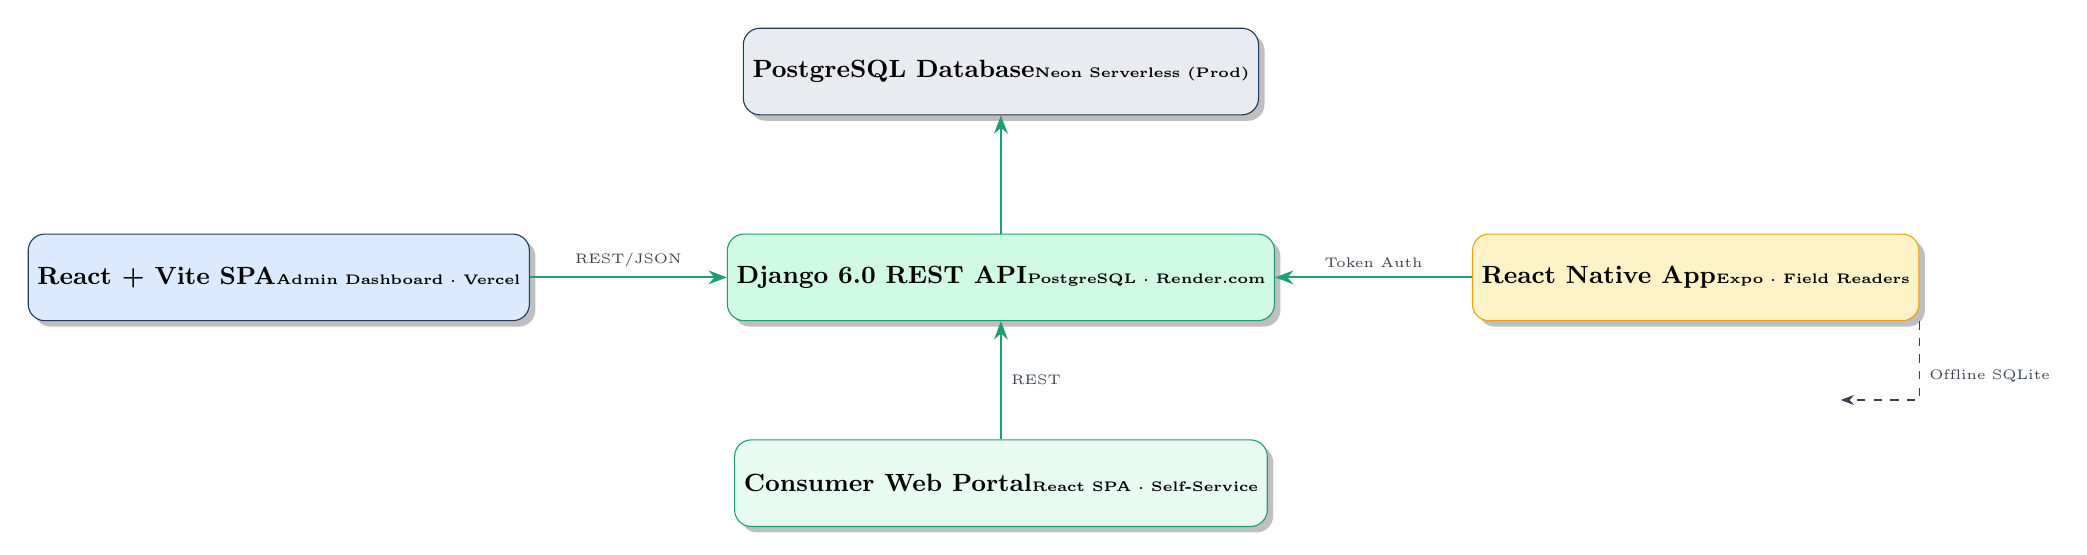
\begin{tikzpicture}[
    node distance=1.8cm,
    box/.style={rectangle, rounded corners=6pt, minimum width=3.2cm, minimum height=1.1cm,
                text centered, font=\small\bfseries, drop shadow},
    arrow/.style={-Stealth, thick, color=primaryGreen},
    dashed_arrow/.style={-Stealth, dashed, color=textMid}
]

% Backend
\node[box, fill=lightGreen, draw=primaryGreen] (backend) {Django 6.0 REST API\\{\tiny PostgreSQL · Render.com}};

% Web SPA
\node[box, fill=lightBlue, draw=deepBlue, left=2.5cm of backend] (web) {React + Vite SPA\\{\tiny Admin Dashboard · Vercel}};

% Mobile App
\node[box, fill=warningBg, draw=accentAmber, right=2.5cm of backend] (mobile) {React Native App\\{\tiny Expo · Field Readers}};

% Consumer Portal
\node[box, fill=lightGreen!50, draw=primaryGreen, below=1.5cm of backend] (consumer) {Consumer Web Portal\\{\tiny React SPA · Self-Service}};

% Database
\node[box, fill=deepBlue!10, draw=deepBlue, above=1.5cm of backend] (db) {PostgreSQL Database\\{\tiny Neon Serverless (Prod)}};

% Arrows
\draw[arrow] (web) -- node[above, font=\tiny, color=textMid]{REST/JSON} (backend);
\draw[arrow] (mobile) -- node[above, font=\tiny, color=textMid]{Token Auth} (backend);
\draw[dashed_arrow] (mobile.south east) -- node[below right, font=\tiny, color=textMid]{Offline SQLite} ++(0,-1) -- ++(-1,0);
\draw[arrow] (consumer) -- node[right, font=\tiny, color=textMid]{REST} (backend);
\draw[arrow] (backend) -- (db);

\end{tikzpicture}
\caption{High-level system architecture of eMeter AMU}
\end{figure}

\section{Technology Stack}

\begin{table}[H]
\centering
\caption{Complete Technology Stack}
\begin{tabularx}{\textwidth}{>{\bfseries}l l X}
\toprule
\textbf{Layer} & \textbf{Technology} & \textbf{Purpose} \\
\midrule
Backend Framework & Django 6.0.2 & REST API, ORM, Admin, Auth \\
Backend Language & Python 3.x & Server-side logic \\
API Framework & Django REST Framework & JSON serialization, Token Auth \\
Primary Database & PostgreSQL (Neon) & Production data store \\
Dev Database & SQLite 3 & Development and testing \\
Frontend Framework & React 18 + Vite & Admin SPA build \\
Frontend Language & TypeScript & Type-safe UI \\
Frontend CSS & Tailwind CSS + shadcn/ui & Component library \\
Mobile Framework & React Native (Expo) & Cross-platform mobile \\
Mobile Local DB & expo-sqlite & Offline SQLite storage \\
Mobile Auth & expo-secure-store & Encrypted token storage \\
PDF Generation & ReportLab (Python) & Bill PDF output \\
Excel Import & openpyxl (Python) & Bulk reading import \\
Excel Export (mobile) & xlsx (JS) & Offline queue export \\
SMS Notifications & Twilio (optional) & Bill SMS alerts \\
Production Hosting & Render.com + Vercel & Cloud deployment \\
\bottomrule
\end{tabularx}
\end{table}

% ============================================================
\chapter{Data Models and Database Schema}
% ============================================================

\section{Overview of Database Models}

All data models reside in \texttt{billing/models.py} in the Django backend. The schema is deployed to PostgreSQL in production and SQLite3 during testing. The following section documents every model, its fields, constraints, and relationships.

\section{User Model}

\begin{actorbox}{\faUser\ \ User — Custom Django Auth Model}
\texttt{billing.User} extends \texttt{AbstractUser} and adds a \texttt{role} field. Every system actor is represented by a \texttt{User} record.
\end{actorbox}

\begin{table}[H]
\centering
\caption{User Model Fields}
\begin{tabularx}{\textwidth}{>{\ttfamily}l l X}
\toprule
\textbf{Field} & \textbf{Type} & \textbf{Description} \\
\midrule
id & BigAutoField & Primary key (auto) \\
username & CharField & Unique login name (inherited from AbstractUser) \\
password & CharField & Hashed password (bcrypt via Django) \\
email & EmailField & User email (optional for staff users) \\
first\_name & CharField & First name \\
last\_name & CharField & Last name \\
is\_active & BooleanField & Whether account is active \\
is\_staff & BooleanField & Access to Django admin panel \\
date\_joined & DateTimeField & Account creation timestamp \\
role & CharField & \textbf{Custom field}: \texttt{admin}, \texttt{meter\_reader}, or \texttt{consumer} \\
\bottomrule
\end{tabularx}
\end{table}

\textbf{Role Choices:}
\begin{featurelist}
    \item \texttt{admin} — Full system access: manage consumers, generate bills, view reports, update settings
    \item \texttt{meter\_reader} — Field access: submit and view readings, view assigned consumers
    \item \texttt{consumer} — Portal access: view own readings and bills, change password
\end{featurelist}

\textbf{Business Rules:}
\begin{featurelist}
    \item Admins cannot log in via the mobile app (\texttt{source: 'mobile'} flag blocks them at API)
    \item Auth tokens are rotated on every login and deleted on logout
    \item Consumers are auto-provisioned a \texttt{User} account when created via the admin panel (username = consumer\_number, default password = consumer\_number)
\end{featurelist}

\section{Meter Model}

\begin{table}[H]
\centering
\caption{Meter Model Fields}
\begin{tabularx}{\textwidth}{>{\ttfamily}l l X}
\toprule
\textbf{Field} & \textbf{Type} & \textbf{Description} \\
\midrule
id & BigAutoField & Primary key \\
meter\_number & CharField (50) & Unique physical meter identifier \\
meter\_type & CharField & \texttt{10} (Standard 10A) or \texttt{25} (Enhanced 25A) \\
status & CharField & \texttt{active}, \texttt{inactive}, or \texttt{disconnected} \\
installation\_date & DateField & Auto-set on creation \\
deactivation\_date & DateField & Nullable — set when meter is retired \\
is\_active & BooleanField & Logical active flag \\
\bottomrule
\end{tabularx}
\end{table}

\section{ConsumerMeterAssignment Model}

Maps which consumer owns which meter during which time period. Prevents duplicate meter assignments, supports meter replacement scenarios, and enforces chronological integrity for readings.

\begin{table}[H]
\centering
\caption{ConsumerMeterAssignment Fields}
\begin{tabularx}{\textwidth}{>{\ttfamily}l l X}
\toprule
\textbf{Field} & \textbf{Type} & \textbf{Description} \\
\midrule
consumer & ForeignKey & Points to \texttt{Consumer} \\
meter & ForeignKey & Points to \texttt{Meter} \\
start\_date & DateField & First date of assignment \\
end\_date & DateField & Last date (null = currently active) \\
is\_active & BooleanField & Whether this is the current assignment \\
assignment\_reason & CharField & \texttt{new\_allocation}, \texttt{quarter\_shift}, \texttt{temporary\_overlap}, \texttt{meter\_replacement} \\
\bottomrule
\end{tabularx}
\end{table}

\textbf{Validation:} On save, overlapping date ranges for the same meter are forbidden and raise a \texttt{ValidationError}.

\section{Consumer Model}

\begin{table}[H]
\centering
\caption{Consumer Model Fields}
\begin{tabularx}{\textwidth}{>{\ttfamily}l l X}
\toprule
\textbf{Field} & \textbf{Type} & \textbf{Description} \\
\midrule
id & BigAutoField & Primary key \\
user & OneToOneField & Optional link to system \texttt{User} (for portal access) \\
consumer\_number & CharField (20) & Unique ID e.g. \texttt{CN012345} \\
name & CharField (100) & Full name \\
email & EmailField & Unique, optional \\
phone & CharField (20) & Contact phone \\
address & TextField & Physical address \\
post & CharField (100) & Job designation / post \\
department & CharField (100) & AMU department \\
meter\_number & CharField (50) & Direct meter reference (legacy) \\
connection\_type & CharField & \texttt{single\_phase} or \texttt{three\_phase} \\
billing\_type & CharField & \texttt{salary} or \texttt{non\_salary} \\
load\_kw & DecimalField & Sanctioned load in kW (default: 1.0 kW) \\
meter\_type & CharField & \texttt{analog}, \texttt{digital}, or \texttt{smart} \\
status & CharField & \texttt{active}, \texttt{inactive}, or \texttt{disconnected} \\
created\_at & DateTimeField & Creation timestamp \\
updated\_at & DateTimeField & Last update timestamp \\
\bottomrule
\end{tabularx}
\end{table}

\section{MeterReading Model}

Records a single physical meter reading event. Enforces strict business rules as database constraints.

\begin{table}[H]
\centering
\caption{MeterReading Model Fields}
\begin{tabularx}{\textwidth}{>{\ttfamily}l l X}
\toprule
\textbf{Field} & \textbf{Type} & \textbf{Description} \\
\midrule
consumer & ForeignKey & Consumer this reading belongs to \\
meter & ForeignKey & The specific meter device read \\
previous\_reading & FloatField & Previous kWh value (auto-set from DB) \\
current\_reading & FloatField & New kWh value entered by reader \\
units\_consumed & FloatField & Auto-computed: current − previous \\
reading\_date & DateField & Date reading was taken \\
reading\_time & TimeField & Time of reading \\
meter\_image & ImageField & Optional photo of meter display \\
remarks & TextField & Reader observations \\
created\_by & ForeignKey & User who submitted this reading \\
created\_at & DateTimeField & DB insertion timestamp \\
created\_source & CharField & \texttt{mobile\_reader}, \texttt{admin\_manual}, \texttt{excel\_import}, \texttt{offline\_sync} \\
manual\_override\_reason & TextField & Justification for manual overrides \\
\bottomrule
\end{tabularx}
\end{table}

\textbf{Validation Rules (enforced in \texttt{clean()} and as DB constraints):}
\begin{enumerate}[leftmargin=1.8em]
    \item A valid \texttt{ConsumerMeterAssignment} must exist for the meter during the reading date
    \item No reading with a later date may already exist for the same meter
    \item \texttt{current\_reading} cannot be less than the chronologically previous reading
    \item Only one reading per meter per calendar month is allowed (duplicate billing-cycle protection)
    \item Minimum 20-day interval between consecutive readings for the same meter
\end{enumerate}

\section{Bill Model}

The financial record of a consumer's electricity charge for a period.

\textbf{Bill Lifecycle:}
\[
\texttt{DRAFT} \rightarrow \texttt{ISSUED} \rightarrow \texttt{PAID}
\]
\[
\texttt{ISSUED} \rightarrow \texttt{CANCELLED} \quad | \quad \texttt{ISSUED} \rightarrow \texttt{OVERDUE}
\]

\begin{table}[H]
\centering
\caption{Bill Model Fields}
\begin{tabularx}{\textwidth}{>{\ttfamily}l l X}
\toprule
\textbf{Field} & \textbf{Type} & \textbf{Description} \\
\midrule
consumer & ForeignKey & Owner of this bill \\
meter & ForeignKey & Meter used for this billing period \\
meter\_reading & ForeignKey & Reading that generated this bill \\
bill\_number & CharField & Auto-generated unique e.g. \texttt{BILL12345678} \\
units & FloatField & kWh consumed this period \\
rate\_per\_unit & FloatField & Tariff rate applied (from BillingSettings) \\
energy\_charges & DecimalField & units × rate \\
fixed\_charges & DecimalField & load\_kw × fixed\_charge\_per\_kw \\
duty\_charge & FloatField & Electricity duty (7.5\% of energy+fixed) \\
regulatory\_surcharge & FloatField & Regulatory levy \\
meter\_rent & FloatField & Phase-1: Rs.10 / Phase-3: Rs.25 \\
arrears & FloatField & Outstanding dues carried forward \\
late\_payment\_surcharge & FloatField & 1.5\% of arrears if arrears > 0 \\
total\_amount & DecimalField & Grand total payable \\
paid\_amount & DecimalField & Amount already received \\
status & CharField & \texttt{draft}, \texttt{issued}, \texttt{paid}, \texttt{overdue}, \texttt{cancelled} \\
is\_locked & BooleanField & True when status = issued — prevents field edits \\
locked\_at & DateTimeField & When bill was finalized \\
locked\_by & ForeignKey & User who finalized the bill \\
units\_consumed\_snapshot & FloatField & Immutable copy of units at finalization \\
rate\_snapshot & FloatField & Immutable copy of rate at finalization \\
total\_amount\_snapshot & FloatField & Immutable copy of total at finalization \\
consumer\_name\_snapshot & CharField & Immutable consumer name at finalization \\
meter\_number\_snapshot & CharField & Immutable meter number at finalization \\
billing\_period\_start & DateField & First day of billing period \\
billing\_period\_end & DateField & Last day of billing period \\
due\_date & DateField & Payment deadline \\
payment\_date & DateField & Date payment was received \\
bill\_date & DateField & Auto-set on creation \\
created\_source & CharField & Origin of this bill \\
\bottomrule
\end{tabularx}
\end{table}

\textbf{Immutability:} Once \texttt{is\_locked = True}, the financial fields (units, rates, amounts, snapshots, billing period) are protected. Any attempt to modify them raises \texttt{ValidationError}.

\section{BillingSettings Model (Singleton)}

\begin{table}[H]
\centering
\caption{BillingSettings Singleton Fields}
\begin{tabularx}{\textwidth}{>{\ttfamily}l l l X}
\toprule
\textbf{Field} & \textbf{Type} & \textbf{Default} & \textbf{Description} \\
\midrule
rate\_per\_unit & FloatField & 8.56 & Rs. per kWh \\
fixed\_charge\_per\_kw & FloatField & 400.0 & Rs. per kW of load \\
phase\_1\_rent & FloatField & 10.0 & Monthly meter rent (1-phase) \\
phase\_3\_rent & FloatField & 25.0 & Monthly meter rent (3-phase) \\
duty\_percentage & FloatField & 7.5 & Electricity duty \% \\
updated\_at & DateTimeField & auto & Last configuration change \\
\bottomrule
\end{tabularx}
\end{table}

\textbf{Note:} Always accessed via \texttt{BillingSettings.get\_settings()} which returns a safe default object if the database is unavailable.

\section{Other Models}

\begin{itemize}[leftmargin=1.5em, itemsep=4pt]
    \item \textbf{Payment} — Records payment transactions against a bill. Fields: \texttt{bill, transaction\_id, amount, payment\_method} (\texttt{credit\_card, debit\_card, bank\_transfer, cash, online}), \texttt{payment\_date, status}.
    \item \textbf{AuditLog} — Immutable trail of all financial actions. Actions: \texttt{reading\_submit, bill\_calculate, bill\_finalize, payment\_update, failed\_mod, pdf\_gen}. Fields: \texttt{user, action, bill, timestamp, details (JSON), ip\_address}.
    \item \textbf{AdminNotification} — In-app notification system. Types: \texttt{info, success, warning, error}. Used for anomaly alerts, sync confirmations, and reading cycle assignments.
\end{itemize}

% ============================================================
\chapter{Actor 1: Administrator}
% ============================================================

\section{Role Definition}

The \textbf{Administrator} is the most privileged actor in the system. Administrators are AMU electricity department staff responsible for managing the entire billing lifecycle, system configuration, and consumer account management. They interact with the system through the \textbf{Web Admin SPA} (React + Vite, hosted on Vercel) and the \textbf{Django Admin Panel}.

\textbf{Technical Identifier:} \texttt{role = 'admin'} on the \texttt{User} model.

\begin{warningbox}
\textbf{Restriction:} Administrators cannot log in via the mobile app. Attempting to do so returns HTTP 403: \textit{``Administrators cannot log in via the mobile app. Please use the Web Dashboard.''}
\end{warningbox}

\section{Authentication}

\begin{actorbox}{Administrator Login Flow}
\begin{enumerate}[leftmargin=1.5em]
    \item Navigate to the Web SPA login page (\texttt{/login})
    \item Submit \texttt{username} and \texttt{password} via \httppost\ \texttt{/api/login/}
    \item Backend validates credentials, checks for rate limiting (5 failed attempts = 5-minute lockout), verifies role
    \item On success: receives \texttt{token} (DRF Token), \texttt{csrftoken}, and \texttt{role} in JSON response
    \item Token stored in browser session; all subsequent requests include \texttt{Authorization: Token <key>} header
    \item Session cookie also created for session-based endpoints
    \item On logout: \httppost\ \texttt{/api/logout/} deletes the token server-side
\end{enumerate}
\end{actorbox}

\section{Module: Dashboard \& Statistics}

\begin{modulebox}{\faChartBar\ \ Admin Dashboard}
Provides real-time KPIs about the electricity billing system.
\end{modulebox}

\textbf{API Endpoint:} \httpget\ \texttt{/api/dashboard-stats/}\\
\textbf{Required Role:} \texttt{admin} or \texttt{meter\_reader}

\textbf{Data Returned:}
\begin{featurelist}
    \item \texttt{total\_consumers} — Total registered consumers
    \item \texttt{total\_bills} — Cumulative bills issued
    \item \texttt{total\_readings} — All meter readings ever submitted
    \item \texttt{total\_revenue} — Sum of all paid bills (in Rs.)
    \item \texttt{pending\_amount} — Sum of all issued-but-unpaid bills
    \item \texttt{current\_month\_units} — Total kWh billed in the current month
\end{featurelist}

\textbf{Frontend:} Page \texttt{Dashboard.tsx} renders stat cards using live API data.

\section{Module: Consumer Management}

\begin{modulebox}{\faUsers\ \ Consumer Management}
Full CRUD for electricity consumers.
\end{modulebox}

\subsection{List Consumers}
\textbf{Endpoint:} \httpget\ \texttt{/api/consumers/}\\
Returns all consumers with their last meter reading value (used to display the ``previous reading'' for billing).

\subsection{Create Consumer}
\textbf{Endpoint:} \httppost\ \texttt{/api/consumers/}\\
\textbf{Required Fields:} \texttt{name}, \texttt{meter\_number}\\
\textbf{Auto-Actions:}
\begin{featurelist}
    \item Generates a unique \texttt{consumer\_number} (format: \texttt{CN} + 6 random digits) if not provided
    \item Normalizes legacy \texttt{connection\_type} values (\texttt{salary} → \texttt{single\_phase}, \texttt{commercial} → \texttt{three\_phase})
    \item Automatically creates a portal User account with \texttt{username = consumer\_number}, \texttt{password = consumer\_number}
    \item Optionally records an \texttt{initial\_reading} as a bootstrap MeterReading
\end{featurelist}

\subsection{View / Edit / Delete Consumer}
\textbf{Endpoint:} \httpget/\httppatch/\httpdelete\ \texttt{/api/consumers/<id>/}\\
\textbf{BOLA Protection:} Role-checked; consumers can only access their own record.

\subsection{Search Consumer}
\textbf{Endpoint:} \httpget\ \texttt{/api/consumers/search/?meter\_number=<query>}\\
Searches by meter number, consumer name, consumer number, or numeric ID.

\subsection{Consumer Portal Account Management}
\begin{featurelist}
    \item \httppost\ \texttt{/api/admin/consumer/<id>/create-portal-account/} — Create portal login for existing consumer (idempotent)
    \item \httppost\ \texttt{/api/admin/consumer/<id>/reset-password/} — Reset consumer password to their consumer number
\end{featurelist}

\textbf{Web UI:} Page \texttt{Consumers.tsx} supports full CRUD, search/filter, status change, and portal account management with an interactive table and slide-out drawer.

\section{Module: Meter Reading Management}

\begin{modulebox}{\faGaugeHigh\ \ Readings Management}
View, add, and import meter readings.
\end{modulebox}

\subsection{View All Readings}
\textbf{Endpoint:} \httpget\ \texttt{/api/readings/?page=<n>\&limit=<n>\&month=<m>\&year=<y>}\\
Supports server-side pagination and filtering by month/year.

\subsection{Submit Reading (Admin Web)}
\textbf{Endpoint:} \httppost\ \texttt{/api/readings/}\\
Allows admin to record a new reading through the web panel (same validation as mobile).

\subsection{Import Readings from Excel}
\textbf{Endpoint:} \httppost\ \texttt{/api/readings/import-excel/}\\
\textbf{Required Role:} \texttt{admin} only\\
\textbf{File size limit:} 5 MB

\textbf{Supported Excel Formats (auto-detected):}
\begin{itemize}[leftmargin=2em]
    \item \textbf{4-column layout} (recommended): Column A = Consumer Number, B = Meter Number, C = Current Reading (kWh), D = Reading Date (optional)
    \item \textbf{3-column layout} (legacy): Column A = Consumer Number, B = Current Reading (kWh), C = Reading Date (optional)
\end{itemize}

\textbf{Processing Pipeline:}
\begin{enumerate}[leftmargin=1.8em]
    \item Peek at row 2 — if column B is numeric → 3-column layout; if text → 4-column layout
    \item Validate consumer number exists in the database
    \item Resolve the active meter assignment for the reading date
    \item Check for duplicate reading in the same billing month for that meter
    \item Validate: current reading ≥ previous reading for that meter
    \item Call \texttt{BillingService.generate\_final\_bill()} atomically for each valid row
    \item Return a summary: \texttt{success\_count}, \texttt{error\_count}, \texttt{duplicate\_count}, \texttt{errors[]}
\end{enumerate}

\subsection{Edit Today's Reading}
\textbf{Endpoint:} \httpput/\httppatch\ \texttt{/api/edit-reading/<id>/}\\
Only permitted if \texttt{reading\_date = today}. Blocked if the reading is linked to a locked bill.

\section{Module: Bill Management}

\begin{modulebox}{\faFileInvoice\ \ Bill Management}
Generate, view, finalize, and manage the payment state of bills.
\end{modulebox}

\subsection{List Bills}
\textbf{Endpoint:} \httpget\ \texttt{/api/bills/?page=<n>\&status=<s>\&accountType=<t>\&startDate=<m>\&endDate=<m>\&search=<q>}

Supports:
\begin{featurelist}
    \item Pagination (default 50 per page)
    \item Text search across bill number, consumer name, consumer number, meter number
    \item Status filter: \texttt{draft, issued, paid, overdue, cancelled}
    \item Account type filter: \texttt{salary} / \texttt{non-salary}
    \item Date range filter by billing period month
    \item Sort by creation date (ascending or descending)
    \item Aggregate summary: total billed, total paid, total pending
\end{featurelist}

\subsection{Manual Bill Generation (Administrative Entry)}
\textbf{Endpoint:} \httppost\ \texttt{/api/bills/manual-generate/}\\
\textbf{Required Role:} \texttt{admin}

Allows an admin to generate a bill for any consumer by providing a current reading value, billing period, and due date. The operation:
\begin{enumerate}[leftmargin=1.8em]
    \item Locks the consumer row (SELECT FOR UPDATE)
    \item Resolves the meter via active assignment
    \item Calls \texttt{BillingService.generate\_final\_bill()} atomically
    \item Records \texttt{created\_source = admin\_manual}
    \item Accepts optional \texttt{manual\_override\_reason} for audit purposes
\end{enumerate}

\subsection{Mark Bill as Paid}
\textbf{Endpoint:} \httppost\ \texttt{/api/bills/<id>/mark-paid/}\\
Only callable on finalized (issued) bills. Sets \texttt{status = paid} and records \texttt{payment\_date}.

\subsection{Mark Bill as Unpaid (Revert)}
\textbf{Endpoint:} \httppost\ \texttt{/api/bills/<id>/mark-unpaid/}\\
\textbf{Required Role:} \texttt{admin} only. Reverts a paid bill back to \texttt{issued} status.

\subsection{Download Bill PDF}
\textbf{Endpoint:} \httpget\ \texttt{/api/bill/<id>/pdf/}

For locked (issued) bills, uses immutable snapshot data to generate the PDF. For draft bills, uses live fields. Uses ReportLab to generate a branded AMU eMeter PDF bill.

\subsection{Send Bill SMS}
\textbf{Endpoint:} \httppost\ \texttt{/api/send-bill-sms/}

If Twilio is configured (\texttt{TWILIO\_ACCOUNT\_SID}, \texttt{TWILIO\_AUTH\_TOKEN} in environment), sends an SMS or WhatsApp message to the consumer's registered phone number containing: bill number, units, amount, and due date.

\section{Module: Billing Calculation Engine}

The \textbf{BillingService} (\texttt{billing/services.py}) contains the authoritative billing calculation logic.

\subsection*{Variable Classification in Bill Generation}

The bill calculation engine relies on two distinct categories of variables to compute the final amount:

\begin{enumerate}[leftmargin=1.8em, itemsep=4pt]
    \item \textbf{Consumer/Meter-Specific Variables (Profile Level):} 
    These are unique to individual consumers or their specific meter connections. They are edited on a per-user basis and generally remain constant across billing cycles. 
    \textit{Examples:} \texttt{load\_kw} (sanctioned load), connection phase type (determines meter rent phase), and consumer position/billing type (\texttt{salary} vs. \texttt{non\_salary}).
    
    \item \textbf{Global Tariff Variables (System Level):} 
    These are general billing parameters applied equally across all consumers. They are managed globally via the \texttt{BillingSettings} singleton and are not associated with any individual meter. They can be updated periodically as utility policies change.
    \textit{Examples:} \texttt{rate\_per\_unit}, \texttt{fixed\_charge\_per\_kw}, \texttt{duty\_percentage}, and \texttt{phase\_1\_rent} / \texttt{phase\_3\_rent}.
\end{enumerate}
\begin{mdframed}[backgroundcolor=codeGray, linecolor=borderColor]
\textbf{Bill Calculation Formula:}\\[0.5em]
\texttt{energy\_charges} = units\_consumed × rate\_per\_unit\\
\texttt{fixed\_charges} = load\_kw × fixed\_charge\_per\_kw\\
\texttt{duty\_charge} = (energy\_charges + fixed\_charges) × (duty\_percentage / 100)\\
\texttt{meter\_rent} = phase\_1\_rent (analog) or phase\_3\_rent (digital/smart)\\
\texttt{late\_payment\_surcharge} = arrears × 0.015 (if arrears > 0)\\[0.5em]
\texttt{total\_amount} = energy + fixed + duty + regulatory + meter\_rent + arrears + late\_payment
\end{mdframed}

\textbf{Atomic Generation Process} (\texttt{BillingService.generate\_final\_bill()}):
\begin{enumerate}[leftmargin=1.8em]
    \item Resolve the active meter assignment for the reading date
    \item Call \texttt{validate\_reading()} — checks all chronological and duplicate constraints
    \item Create \texttt{MeterReading} record
    \item Create \texttt{Bill} with \texttt{status = draft}
    \item Call \texttt{calculate\_bill()} — applies tariff from \texttt{BillingSettings}
    \item Populate all immutable snapshot fields
    \item Lock the bill: \texttt{is\_locked = True}, \texttt{status = issued}
    \item Write \texttt{AuditLog} entry
\end{enumerate}

\textbf{Real-time Estimate API:} \httppost\ \texttt{/api/calculate-estimate/}\\
Returns a full line-item breakdown without saving anything. Used by the mobile app to show a live cost preview as the reader types the reading value.

\section{Module: Reports}

\textbf{Endpoint:} \httpget\ \texttt{/api/reports-data/}\\
\textbf{Required Role:} \texttt{admin}

Returns chart-ready data:
\begin{featurelist}
    \item \textbf{Top 10 Consumers by Usage} — Consumer names and total kWh billed
    \item \textbf{Monthly Usage (last 6 months)} — Trend data for usage bar chart
    \item \textbf{Revenue Breakdown} — Salary vs. Non-Salary revenue split
\end{featurelist}

Frontend page \texttt{Reports.tsx} renders these as interactive charts.

\section{Module: System Settings}

\begin{modulebox}{\faCog\ \ Billing Settings}
Administrator-only control over global tariff rates.
\end{modulebox}

\begin{featurelist}
    \item \httpget\ \texttt{/api/settings/} — Retrieve current tariff configuration
    \item \httppost\ \texttt{/api/settings/update/} — Update rate\_per\_unit, fixed\_charge\_per\_kw, phase rents, duty percentage
\end{featurelist}

Changes take effect immediately for all future bill calculations.

\section{Module: Reading Cycle Management}

\textbf{Endpoint:} \httppost\ \texttt{/api/start-reading-cycle/}

Admin can initiate a new monthly reading cycle for a zone and notify all meter readers. The system creates \texttt{AdminNotification} records for every user with \texttt{role = meter\_reader}.

\section{Module: Mobile Data Export (Offline Sync File)}

\textbf{Endpoint:} \httpget\ \texttt{/api/admin/export-mobile-sync/}\\
\textbf{Required Role:} \texttt{admin}

Generates and downloads a JSON file containing:
\begin{featurelist}
    \item All active consumers with their last reading values and billing settings
    \item Current \texttt{BillingSettings} (rate\_per\_unit, fixed\_charge\_per\_kw, duty\_percentage, meter rents)
\end{featurelist}

This file is used by field meter readers to seed their offline SQLite database when internet is not available.

\section{Module: Notifications}

\begin{featurelist}
    \item \httpget\ \texttt{/api/notifications/} — Retrieve notifications for the logged-in user (last 100)
    \item \httppost\ \texttt{/api/notifications/mark-read/} — Mark one or all notifications as read
\end{featurelist}

Notifications are automatically created for:
\begin{featurelist}
    \item Successful mobile sync of readings
    \item Bulk Excel import completion
    \item Consumption anomaly detection (reading 200\%+ above 3-month rolling average)
    \item New reading cycle start events
\end{featurelist}

\textbf{Anomaly Detection Logic:}\\
After each reading submission, \texttt{check\_consumption\_anomaly()} computes the 3-month rolling average of the consumer's past readings. If current usage exceeds average by more than 200\%, an \texttt{error}-type notification is created flagging potential leakage or faulty reading.

\section{Module: Web Admin Panel (Django Admin)}

Django's built-in admin panel is configured in \texttt{billing/admin.py} and accessible at \texttt{/admin/}. Superusers can directly manage all database records, including:
\begin{featurelist}
    \item Full CRUD for all models
    \item Bulk actions on bills and readings
    \item User management and password reset
    \item Raw audit log inspection
\end{featurelist}

\section{Web SPA Pages Summary}

\begin{table}[H]
\centering
\caption{Admin Web SPA Pages}
\begin{tabularx}{\textwidth}{>{\ttfamily}l l X}
\toprule
\textbf{Route / Component} & \textbf{Access} & \textbf{Functionality} \\
\midrule
/dashboard & admin, reader & KPI stats, quick links \\
/consumers & admin, reader & Consumer CRUD, search, filter \\
/readings & admin, reader & Readings list, submit, import Excel \\
/billing & admin & Bills list, PDF, mark paid, manual generate \\
/reports & admin & Chart-based usage reports \\
/settings & admin & Tariff configuration \\
/consumer-login & consumer & Consumer self-service login \\
/consumer-dashboard & consumer & Consumer portal home \\
/consumer-bills & consumer & Consumer bill list + PDF \\
/consumer-readings & consumer & Consumer reading history \\
\bottomrule
\end{tabularx}
\end{table}

% ============================================================
\chapter{Actor 2: Meter Reader}
% ============================================================

\section{Role Definition}

The \textbf{Meter Reader} is a field staff member who physically visits each consumer's location on campus to record electricity meter readings. The primary tool is the \textbf{eMeter Mobile App} (React Native/Expo) running on an Android or iOS smartphone. The system supports two distinct operational modes: \textbf{Online Mode} and \textbf{Offline Mode}.

\textbf{Technical Identifier:} \texttt{role = 'meter\_reader'} on the \texttt{User} model.

\section{Authentication}

\begin{actorbox}{Meter Reader Login Flow}
\begin{enumerate}[leftmargin=1.5em]
    \item Open the mobile app and enter username and password on \texttt{LoginScreen.js}
    \item \httppost\ \texttt{/api/login/} with \texttt{source: 'mobile'} flag
    \item Backend validates credentials and role (returns 403 if user is admin)
    \item Receives DRF Token — stored encrypted in \texttt{expo-secure-store}
    \item User object stored in \texttt{AsyncStorage} for offline context
    \item On logout: token deleted from SecureStore, server-side token destroyed, SQLite consumer cache preserved
\end{enumerate}
\end{actorbox}

\textbf{401 Auto-Recovery:} An Axios response interceptor automatically clears stale tokens on 401 responses.

\section{Mobile App Screen Architecture}

\begin{table}[H]
\centering
\caption{Mobile App Screens}
\begin{tabularx}{\textwidth}{>{\ttfamily}l l X}
\toprule
\textbf{Screen} & \textbf{File} & \textbf{Primary Purpose} \\
\midrule
LoginScreen & LoginScreen.js & Authentication \\
DashboardScreen & DashboardScreen.js & Home hub, stats, sync controls \\
SearchScreen & SearchScreen.js & Find consumer to read \\
SubmitReadingScreen & SubmitReadingScreen.js & Enter and submit meter reading \\
BillPreviewScreen & BillPreviewScreen.js & View generated bill post-submission \\
HistoryScreen & HistoryScreen.js & Past readings for a consumer \\
SettingsScreen & SettingsScreen.js & App preferences, logout \\
AddConsumerScreen & AddConsumerScreen.js & Add consumer (admin only) \\
\bottomrule
\end{tabularx}
\end{table}

\section{Module: Dashboard Screen}

The Dashboard is the meter reader's home screen. It shows:

\subsection{Statistics Section}
\begin{featurelist}
    \item \textbf{Total Consumers} — from API dashboard stats
    \item \textbf{Total Readings} — cumulative reading count
    \item \textbf{Total Sync Online} — readings confirmed by server
    \item \textbf{Unsynced Readings} — count from local SQLite offline queue
\end{featurelist}

\subsection{Daily Sync Tracker}
An interactive progress bar showing how many readings have been synced vs. the reader's daily target goal. The target (default: 15) can be customized by tapping the card and entering a new number.

\subsection{Offline Queue Banner}
When there are pending local readings, a yellow banner appears showing the count. Buttons on the banner allow:
\begin{featurelist}
    \item \textbf{Excel} — Export offline readings as a spreadsheet for admin import
    \item \textbf{Sync} — Push all pending readings to the server
\end{featurelist}

\subsection{Quick Actions Grid}
Six action buttons:
\begin{enumerate}[leftmargin=1.8em]
    \item \textbf{Search \& Submit} — Go to consumer search screen
    \item \textbf{Reading History} — View chronological reading history
    \item \textbf{Queue Inspector} — View/delete items in offline queue
    \item \textbf{Pull Registry} — Download latest consumer list from server to SQLite
    \item \textbf{Import Data} — Import admin-generated JSON sync file
    \item \textbf{Push Sync Queue} — Push all offline readings to server
\end{enumerate}

\subsection{Recent Activity Feed}
A chronological log of recent actions (last 8 entries) stored in \texttt{AsyncStorage}. Includes timestamps and action descriptions.

\subsection{Notifications}
Bell icon with badge count. Tapping opens a modal with server-side notifications (sync confirmations, anomaly alerts, reading cycle assignments).

\section{Module: Consumer Search}

\textbf{Screen:} \texttt{SearchScreen.js}

\begin{actorbox}{Search Flow (Online + Offline)}
\textbf{Online Mode:}
\begin{enumerate}
    \item User types in search box (debounced 300ms)
    \item Calls \httpget\ \texttt{/api/consumers/search/?meter\_number=<query>}
    \item Results display: name, consumer number, meter number, previous reading, status
    \item Tap a result → navigate to \texttt{SubmitReadingScreen}
\end{enumerate}

\vspace{0.5em}
\textbf{Offline Mode:}
\begin{enumerate}
    \item Falls back to \texttt{searchConsumersOffline()} — SQLite LIKE query on \texttt{consumers} table
    \item Search fields: name, consumer\_number, meter\_number
    \item Tap result → navigate to \texttt{SubmitReadingScreen} with cached consumer data
\end{enumerate}
\end{actorbox}

\section{Module: Reading Submission}

\textbf{Screen:} \texttt{SubmitReadingScreen.js}

This is the core functionality of the meter reader's workflow.

\begin{actorbox}{Submit Reading — Dual-Mode Flow}

\textbf{Step 1 — Restore Pending Reading (on screen open):}\\
Checks the offline queue for any existing pending reading for this consumer today. If found, pre-fills the reading value (prevents double entry).

\vspace{0.5em}
\textbf{Step 2 — Live Estimate (as user types):}\\
After a 600ms debounce:
\begin{itemize}
    \item Online: Calls \httppost\ \texttt{/api/calculate-estimate/} for server-computed breakdown
    \item Offline: Falls back to \texttt{calculateOfflineEstimate()} using local SQLite billing settings
\end{itemize}
Displays: Energy Charges, Fixed Charges, Duty, Meter Rent, and Grand Total estimate.

\vspace{0.5em}
\textbf{Step 3 — Submit Button:}
\begin{enumerate}
    \item \textbf{Always save locally first:} Calls \texttt{saveOfflineReading()} → inserts into SQLite \texttt{meter\_readings} table with \texttt{status = pending\_create}
    \item \textbf{Try online submit:} Calls \httppost\ \texttt{/api/reading-and-bill/}
    \item On success: marks local copy as \texttt{synced}, fetches full bill detail, navigates to \texttt{BillPreviewScreen}
    \item On network failure: shows Alert ``Reading saved locally. Will sync when back online.'', returns to search screen
    \item On server validation error: shows specific error message (e.g., ``duplicate billing cycle'')
\end{enumerate}
\end{actorbox}

\textbf{Validation (client-side):}
\begin{featurelist}
    \item Current reading must be a valid number
    \item Current reading ≥ previous reading
    \item Empty reading field shows clear error
\end{featurelist}

\section{Module: Bill Preview}

\textbf{Screen:} \texttt{BillPreviewScreen.js}

Displays the generated bill after a successful reading submission:
\begin{featurelist}
    \item Bill number, consumer details, meter number, billing period
    \item Reading values: previous, current, units consumed
    \item Full charge breakdown: energy, fixed, duty, meter rent, regulatory surcharge, arrears, late payment
    \item Grand total in large text
    \item Option to share/view the PDF bill
    \item Option to send SMS notification to consumer
\end{featurelist}

\section{Module: Reading History}

\textbf{Screen:} \texttt{HistoryScreen.js}

Displays a chronological list of all readings submitted by the current meter reader (or for a specific consumer). Supports:
\begin{featurelist}
    \item Pagination with ``Load More'' functionality
    \item Filter by month/year
    \item View synced vs. offline-pending status
    \item Export filtered results to Excel spreadsheet
\end{featurelist}

\section{Module: Offline Data Management}

The offline system is powered by a local SQLite database (\texttt{emeter.db}) managed by \texttt{expo-sqlite} with a migration system.

\subsection{SQLite Schema}

\begin{table}[H]
\centering
\caption{Mobile SQLite Tables}
\begin{tabularx}{\textwidth}{>{\ttfamily}l X}
\toprule
\textbf{Table} & \textbf{Columns \& Purpose} \\
\midrule
consumers & id, consumer\_number, name, email, phone, address, meter\_number, meter\_type, load\_kw, previous\_reading, status — Local consumer registry \\
meter\_readings & id (TEXT), consumer\_id, consumer\_number, consumer\_name, meter\_number, current\_reading, previous\_reading, reading\_date, status (pending\_create / synced / conflict), last\_error, saved\_at — Offline queue \\
billing\_settings & id, rate\_per\_unit, fixed\_charge\_per\_kw, duty\_percentage, phase\_1\_rent, phase\_3\_rent, surcharge\_percentage — Local billing parameters \\
users & id, username, name, password\_hash — Offline user cache \\
\bottomrule
\end{tabularx}
\end{table}

\subsection{Registry Pull (Online → Offline)}
\textbf{Action:} ``Pull Registry'' button on Dashboard.\\
Calls \texttt{pullRegistryFromServer()} which:
\begin{enumerate}[leftmargin=1.8em]
    \item Fetches all consumers from \texttt{/api/consumers/}
    \item Fetches billing settings from \texttt{/api/settings/}
    \item Upserts both into local SQLite (INSERT OR REPLACE)
\end{enumerate}

\subsection{JSON Sync File Import (Total Offline Mode)}
\textbf{Action:} ``Import Data'' button on Dashboard.\\
Meter reader selects a \texttt{.json} file exported from the admin panel. \texttt{importSyncFile()} parses the file and:
\begin{enumerate}[leftmargin=1.8em]
    \item Validates \texttt{version} and \texttt{consumers} fields exist
    \item Calls \texttt{cacheConsumersToDb()} to upsert all consumers
    \item Calls \texttt{cacheBillingSettings()} to store tariff values locally
\end{enumerate}

\subsection{Offline Queue Push (Offline → Online)}
\textbf{Action:} ``Sync'' button or automatic on next online session.\\
\texttt{pushOfflineQueueToServer()} iterates all \texttt{pending\_create} readings:
\begin{featurelist}
    \item Calls \texttt{submitReadingAndBillAPI()} for each reading
    \item On success: marks local record \texttt{synced}, updates \texttt{previous\_reading} in local consumers table
    \item On ``already exists'' error: treats as success (network re-delivery scenario)
    \item On other errors: marks as \texttt{conflict}, stores \texttt{last\_error} message
    \item Returns \texttt{\{synced, failed, errors[]\}} summary
\end{featurelist}

\subsection{Export Offline Queue to Excel}
Allows a meter reader to export their offline queue as an \texttt{.xlsx} file for manual delivery to admin. Columns: Consumer Number, Consumer Name, Meter Number, Current Reading, Previous Reading, Units Consumed, Reading Date, Sync Status.

\section{Module: App Settings}

\textbf{Screen:} \texttt{SettingsScreen.js}

\begin{featurelist}
    \item Theme toggle (light/dark mode) — stored in \texttt{AsyncStorage}
    \item Display current user information (name, role, username)
    \item Logout button — clears auth token and user session
    \item App version display
\end{featurelist}

\section{Meter Reader Web Access}

Meter readers also have access to the Web Admin SPA with a restricted permission set:
\begin{featurelist}
    \item View dashboard statistics
    \item Submit readings via web panel (\texttt{Readings.tsx} page shows ``New Reading'' button for non-admins)
    \item View consumer list and reading history
    \item Access their own notifications
\end{featurelist}

They \textbf{cannot}: generate bills manually, import Excel, modify billing settings, manage consumers, or view financial reports.

% ============================================================
\chapter{Actor 3: Consumer (Self-Service Portal)}
% ============================================================

\section{Role Definition}

The \textbf{Consumer} is an AMU electricity customer who can log into a dedicated self-service web portal to view their own billing history, meter readings, and download bills. Consumers have read-only access to their own data and cannot affect any other records.

\textbf{Technical Identifier:} \texttt{role = 'consumer'} on the \texttt{User} model.

\section{Account Provisioning}

Consumer accounts are created in two ways:
\begin{enumerate}[leftmargin=1.8em]
    \item \textbf{Automatic:} When admin creates a consumer via \texttt{POST /api/consumers/}, a User is auto-created with \texttt{username = consumer\_number} and \texttt{password = consumer\_number}
    \item \textbf{Manual:} Admin uses \texttt{POST /api/admin/consumer/<id>/create-portal-account/} to explicitly create the account
\end{enumerate}

Default credentials: \texttt{username = consumer\_number}, \texttt{password = consumer\_number}. Consumers are expected to change their password on first login.

\section{Authentication}

The consumer portal is accessible from the React SPA at \texttt{/consumer-login}. Authentication uses the same \texttt{/api/login/} endpoint. The \texttt{role} field returned in the response determines that the user sees the consumer portal layout.

\section{Module: Consumer Profile (My Account)}

\textbf{Endpoint:} \httpget\ \texttt{/api/consumer/portal/me/}\\
\textbf{Required Role:} \texttt{consumer}

Returns the consumer's own record:
\begin{featurelist}
    \item Consumer number, name, meter number
    \item Email, phone, address
    \item Connection type (\texttt{single\_phase} / \texttt{three\_phase})
    \item Billing type (\texttt{salary} / \texttt{non\_salary})
    \item Account status
\end{featurelist}

\textbf{Web UI:} \texttt{ConsumerDashboard.tsx} shows a profile card with this data alongside stats (current bill, usage comparison, payment history).

\section{Module: View Meter Readings}

\textbf{Endpoint:} \httpget\ \texttt{/api/consumer/portal/readings/?page=<n>\&page\_size=<n>}\\
\textbf{Required Role:} \texttt{consumer}

Returns paginated list of the consumer's own meter readings:
\begin{featurelist}
    \item Reading date
    \item Previous reading value (kWh)
    \item Current reading value (kWh)
    \item Units consumed
    \item Remarks/notes from the reader
\end{featurelist}

\textbf{Web UI:} \texttt{ConsumerReadings.tsx} shows a filterable, paginated table with month-to-month usage trend.

\section{Module: View Bills}

\textbf{Endpoint:} \httpget\ \texttt{/api/consumer/portal/bills/?page=<n>\&page\_size=<n>}\\
\textbf{Required Role:} \texttt{consumer}

Returns paginated list of the consumer's bills with complete detail:
\begin{featurelist}
    \item Bill number, bill date, billing period start and end
    \item Due date and payment status
    \item Full charge breakdown: energy charges, fixed charges, duty, meter rent, regulatory surcharge, arrears, late payment surcharge
    \item Total amount, paid amount
    \item \texttt{is\_paid} boolean flag
    \item Consumer's meter info, address, connection type, load kW
\end{featurelist}

\textbf{Web UI:} \texttt{ConsumerBills.tsx} shows bills in a card/table layout with colored status badges (paid/issued/overdue).

\subsection{Download Bill PDF}
Consumers can download their own bill PDFs via \httpget\ \texttt{/api/bill/<id>/pdf/}.\\
\textbf{BOLA Protection:} The endpoint verifies \texttt{bill.consumer.user == request.user} before serving the PDF. Accessing another consumer's bill returns HTTP 403.

\section{Module: Change Password}

\textbf{Endpoint:} \httppost\ \texttt{/api/consumer/portal/change-password/}\\
\textbf{Required Role:} \texttt{consumer}

Required fields: \texttt{old\_password}, \texttt{new\_password}, \texttt{confirm\_password}

Validation:
\begin{featurelist}
    \item All three fields must be present
    \item New password and confirmation must match
    \item New password must be at least 6 characters
    \item Old password must be correct (verified via Django's \texttt{check\_password})
\end{featurelist}

On success: existing auth token is invalidated (deleted), consumer must re-login.

\textbf{Web UI:} \texttt{ConsumerChangePassword.tsx} provides a form with show/hide password toggles and validation messages.

\section{Consumer Portal Security Model}

All consumer portal endpoints enforce the following security measures:
\begin{featurelist}
    \item Role restriction via \texttt{@require\_role('consumer')} decorator — returns HTTP 403 if non-consumer tries to access
    \item Data isolation: all queries are filtered to \texttt{consumer = request.user.consumer\_profile}
    \item BOLA/IDOR protection on PDF download: bill ownership is verified before serving
    \item Token invalidation on password change prevents session hijacking after credential updates
\end{featurelist}

% ============================================================
\chapter{Actor 4: Django Superuser / System Administrator}
% ============================================================

\section{Role Definition}

The \textbf{Django Superuser} is a technical administrator with full access to Django's built-in admin panel (\texttt{/admin/}). This role is distinct from the application-level \texttt{admin} role and is typically held by the system developer or IT administrator.

\section{Capabilities}

\begin{featurelist}
    \item Full CRUD access to all database tables through the Django Admin interface
    \item Create and manage all user accounts (including setting \texttt{role} field)
    \item Directly query and modify \texttt{BillingSettings}, \texttt{AuditLog}, \texttt{Payment} records
    \item Force-reset any user's password
    \item Access database migration management
    \item View raw server logs
\end{featurelist}

\section{Creation}

A superuser is created via the command line:
\begin{lstlisting}[language=bash]
# From the electricity_system directory:
python create_superuser.py
# or
python manage.py createsuperuser
\end{lstlisting}

The project provides \texttt{create\_admin.py} and \texttt{create\_superuser.py} scripts for initial setup.

\section{Admin Panel Registration}

The following models are registered in \texttt{billing/admin.py} with custom configurations:
\begin{featurelist}
    \item \textbf{User} — with role filter, search by username/email
    \item \textbf{Consumer} — with status/billing\_type filters, search by name/consumer\_number/meter\_number
    \item \textbf{MeterReading} — with date filters, consumer search
    \item \textbf{Bill} — with status/created\_source filters, locking indicator
    \item \textbf{Payment} — with method/status filters
    \item \textbf{AuditLog} — read-only view with action/user filters
    \item \textbf{BillingSettings} — singleton editor
    \item \textbf{Meter} — with status/type filters
    \item \textbf{ConsumerMeterAssignment} — assignment history view
    \item \textbf{AdminNotification} — notification management
\end{featurelist}

% ============================================================
\chapter{Cross-Cutting Concerns}
% ============================================================

\section{Authentication Architecture}

The system uses a dual-authentication strategy:

\begin{table}[H]
\centering
\caption{Authentication Methods by Actor}
\begin{tabularx}{\textwidth}{>{\bfseries}l l X}
\toprule
\textbf{Actor} & \textbf{Method} & \textbf{Storage} \\
\midrule
Admin (Web) & DRF Token + Session & Session cookie (HttpOnly) + Token in memory \\
Meter Reader (Mobile) & DRF Token & expo-secure-store (encrypted on device) \\
Consumer (Web Portal) & DRF Token + Session & Session cookie \\
Superuser & Django Session & Browser session cookie \\
\bottomrule
\end{tabularx}
\end{table}

\section{Authorization Decorators}

Two custom decorators in \texttt{electricity\_system/authentication.py}:

\begin{featurelist}
    \item \texttt{@require\_authenticated} — Returns JSON 401 if user is not logged in
    \item \texttt{@require\_role('admin', 'meter\_reader')} — Returns JSON 403 if user's role is not in the allowed list
\end{featurelist}

Three DRF permission classes in \texttt{billing/permissions.py}:
\begin{featurelist}
    \item \texttt{IsAdminUser} — Admin role only
    \item \texttt{IsMeterReader} — Admin or meter\_reader
    \item \texttt{IsOwnerOrAdmin} — Object-level: owner or admin
\end{featurelist}

\section{Rate Limiting}

Login attempts are rate-limited per IP address using Django's cache framework:
\begin{featurelist}
    \item After 5 failed login attempts from the same IP within 5 minutes → HTTP 429 (Too Many Requests)
    \item Cache key: \texttt{login\_attempts\_<ip>}
    \item On successful login: failed attempt counter is cleared
\end{featurelist}

\section{Security Measures}

\begin{table}[H]
\centering
\caption{Security Controls by Feature}
\begin{tabularx}{\textwidth}{>{\bfseries}l X}
\toprule
\textbf{Control} & \textbf{Implementation} \\
\midrule
CSRF Protection & Django CSRF middleware; cookie-based for web SPA; exempt for token-authenticated mobile \\
HTTPS Enforcement & HSTS headers, SSL redirect via Render.com in production \\
CORS Policy & Explicit whitelist only; \texttt{CORS\_ALLOW\_ALL\_ORIGINS = False} \\
Session Security & HttpOnly session cookies, SameSite=Lax (dev) / None (prod) \\
Token Rotation & Auth token recreated on every login, destroyed on logout/password change \\
Bill Immutability & Protected fields raise \texttt{ValidationError} when locked bill is modified \\
BOLA/IDOR Protection & All consumer-scoped endpoints verify ownership before data access \\
Admin/Mobile Separation & Admin login via mobile returns HTTP 403 \\
\bottomrule
\end{tabularx}
\end{table}

\section{Logging and Audit Trail}

\begin{featurelist}
    \item \textbf{Application Logging:} Django rotating file handler at \texttt{logs/emeter.log} (10 MB, 5 backup files, ERROR level)
    \item \textbf{Audit Log:} Every significant financial action writes to \texttt{AuditLog} table including user identity, action type, bill reference, timestamp, IP address, and a JSON details payload
\end{featurelist}

\section{PDF Bill Generation}

The \texttt{BillPDFGenerator} class in \texttt{billing/pdf\_generator.py} uses the \textbf{ReportLab} library to produce branded PDF bills with:
\begin{featurelist}
    \item AMU eMeter header with logo
    \item Consumer details section
    \item Meter reading values (previous, current, units)
    \item Complete charge breakdown table
    \item Total payable amount (rounded to nearest rupee)
    \item Due date and bill number
    \item Finalization watermark for locked bills
\end{featurelist}

For locked bills, snapshot data is used to ensure the PDF is immutable. For draft bills, live values are used with a ``draft'' indicator.

% ============================================================
\chapter{API Reference Summary}
% ============================================================

\section{Complete API Endpoint Listing}

\begin{longtable}{>{\ttfamily}p{0.36\textwidth} p{0.08\textwidth} p{0.12\textwidth} p{0.32\textwidth}}
\caption{All API Endpoints} \\
\toprule
\textbf{Endpoint} & \textbf{Method} & \textbf{Role} & \textbf{Description} \\
\midrule
\endfirsthead
\multicolumn{4}{c}{\textit{Table continued\ldots}} \\
\toprule
\textbf{Endpoint} & \textbf{Method} & \textbf{Role} & \textbf{Description} \\
\midrule
\endhead
\midrule \multicolumn{4}{r}{\textit{Continued on next page}} \\
\endfoot
\bottomrule
\endlastfoot

/api/login/ & POST & Any & Authenticate user, receive token \\
/api/logout/ & POST & Auth & Destroy token, end session \\
/api/me/ & GET & Auth & Get current user info \\
/api/profile/update/ & POST & Auth & Update user profile \\
/api/csrf/ & GET & Any & Get CSRF token \\
/api/health/ & GET & Any & Health check \\
\midrule
/api/dashboard-stats/ & GET & Admin/Reader & KPI statistics \\
/api/reports-data/ & GET & Admin & Chart data for reports \\
/api/settings/ & GET & Admin/Reader & Get billing settings \\
/api/settings/update/ & POST & Admin & Update billing settings \\
\midrule
/api/consumers/ & GET & Admin/Reader & List all consumers \\
/api/consumers/ & POST & Admin/Reader & Create consumer \\
/api/consumers/<id>/ & GET & Admin/Reader & Get consumer details \\
/api/consumers/<id>/ & PATCH & Admin/Reader & Update consumer \\
/api/consumers/<id>/ & DELETE & Admin/Reader & Delete consumer \\
/api/consumers/search/ & GET & Auth & Search consumers \\
/api/consumer/<id>/readings/ & GET & Auth & Consumer's reading history \\
\midrule
/api/readings/ & GET & Admin/Reader & List all readings \\
/api/readings/ & POST & Admin/Reader & Submit a reading \\
/api/readings/import-excel/ & POST & Admin & Bulk import from Excel \\
/api/submit-reading/ & POST & Admin/Reader & Submit reading only \\
/api/reading-and-bill/ & POST & Admin/Reader & Submit reading + generate bill \\
/api/edit-reading/<id>/ & PUT/PATCH & Admin/Reader & Edit today's reading \\
/api/calculate-estimate/ & POST & Admin/Reader & Live bill estimate \\
\midrule
/api/bills/ & GET & Admin/Reader & List bills with filters \\
/api/bill/<id>/ & GET & Auth & Get bill details \\
/api/bill/<id>/ & PATCH & Admin/Reader & Update bill status \\
/api/bill/<id>/pdf/ & GET & Auth & Download bill PDF \\
/api/bills/<id>/mark-paid/ & POST & Admin/Reader & Mark bill as paid \\
/api/bills/<id>/mark-unpaid/ & POST & Admin & Revert to unpaid \\
/api/bills/manual-generate/ & POST & Admin & Admin manual bill \\
/api/send-bill-sms/ & POST & Admin/Reader & Send SMS notification \\
\midrule
/api/notifications/ & GET & Admin/Reader & Get notifications \\
/api/notifications/mark-read/ & POST & Admin/Reader & Mark as read \\
/api/start-reading-cycle/ & POST & Admin & Start monthly cycle \\
\midrule
/api/consumer/portal/me/ & GET & Consumer & Own profile \\
/api/consumer/portal/readings/ & GET & Consumer & Own readings \\
/api/consumer/portal/bills/ & GET & Consumer & Own bills \\
/api/consumer/portal/change-password/ & POST & Consumer & Change password \\
\midrule
/api/admin/consumer/<id>/create-portal-account/ & POST & Admin & Create consumer login \\
/api/admin/consumer/<id>/reset-password/ & POST & Admin & Reset consumer password \\
/api/admin/export-mobile-sync/ & GET & Admin & Export offline JSON file \\

\end{longtable}

% ============================================================
\chapter{Deployment Configuration}
% ============================================================

\section{Environment Variables}

\begin{table}[H]
\centering
\caption{Required Environment Variables}
\begin{tabularx}{\textwidth}{>{\ttfamily\raggedright\arraybackslash}p{0.45\textwidth} l X}
\toprule
\textbf{Variable} & \textbf{Context} & \textbf{Purpose} \\
\midrule
DJANGO\_SECRET\_KEY & Backend & Django secret key (required in production) \\
DATABASE\_URL & Backend & Neon PostgreSQL connection URL \\
DB\_ENGINE / DB\_NAME / DB\_USER / DB\_PASSWORD / DB\_HOST / DB\_PORT & Backend & Individual DB settings (override by DATABASE\_URL) \\
ALLOWED\_HOSTS & Backend & Comma-separated allowed hostnames \\
CORS\_ALLOWED\_ORIGINS\_EXTRA & Backend & Comma-separated extra CORS origins \\
DEBUG & Backend & \texttt{True} for dev, \texttt{False} for prod \\
TWILIO\_ACCOUNT\_SID & Backend & Twilio SMS account ID (optional) \\
TWILIO\_AUTH\_TOKEN & Backend & Twilio API token (optional) \\
TWILIO\_PHONE\_NUMBER & Backend & Twilio sender number (optional) \\
TWILIO\_WHATSAPP\_FROM & Backend & Twilio WhatsApp sender (optional) \\
EXPO\_PUBLIC\_API\_URL & Mobile & Backend server base URL \\
VITE\_API\_URL & Web SPA & Backend server base URL \\
\bottomrule
\end{tabularx}
\end{table}

\section{Production Deployment}

\begin{itemize}[leftmargin=1.5em, itemsep=4pt]
    \item \textbf{Backend:} Deployed on Render.com using \texttt{render.yaml}. Uses \texttt{gunicorn} as WSGI server (see \texttt{Procfile}). Static files served via WhiteNoise.
    \item \textbf{Database:} Neon Serverless PostgreSQL. SSL required.
    \item \textbf{Web SPA:} Deployed on Vercel. \texttt{vercel.json} configures all routes to serve \texttt{index.html} (SPA routing).
    \item \textbf{Mobile App:} Built with Expo EAS (Expo Application Services). \texttt{eas.json} defines build profiles for development, preview, and production.
\end{itemize}

\section{Running Locally}

\begin{lstlisting}[language=bash]
# 1. Start the Django backend
cd electricity_system
python manage.py runserver 0.0.0.0:8000

# 2. Start the Web Admin SPA
cd energy-hub-ui
npm run dev

# 3. Start the Mobile App (requires Expo CLI)
cd eMeterApp
npx expo start

# All-in-one (using the startup script from project root)
./START_PROJECT.sh
\end{lstlisting}

% ============================================================
\chapter{Data Flow Diagrams}
% ============================================================

\section{Online Reading Submission Flow}

\begin{figure}[H]
\centering
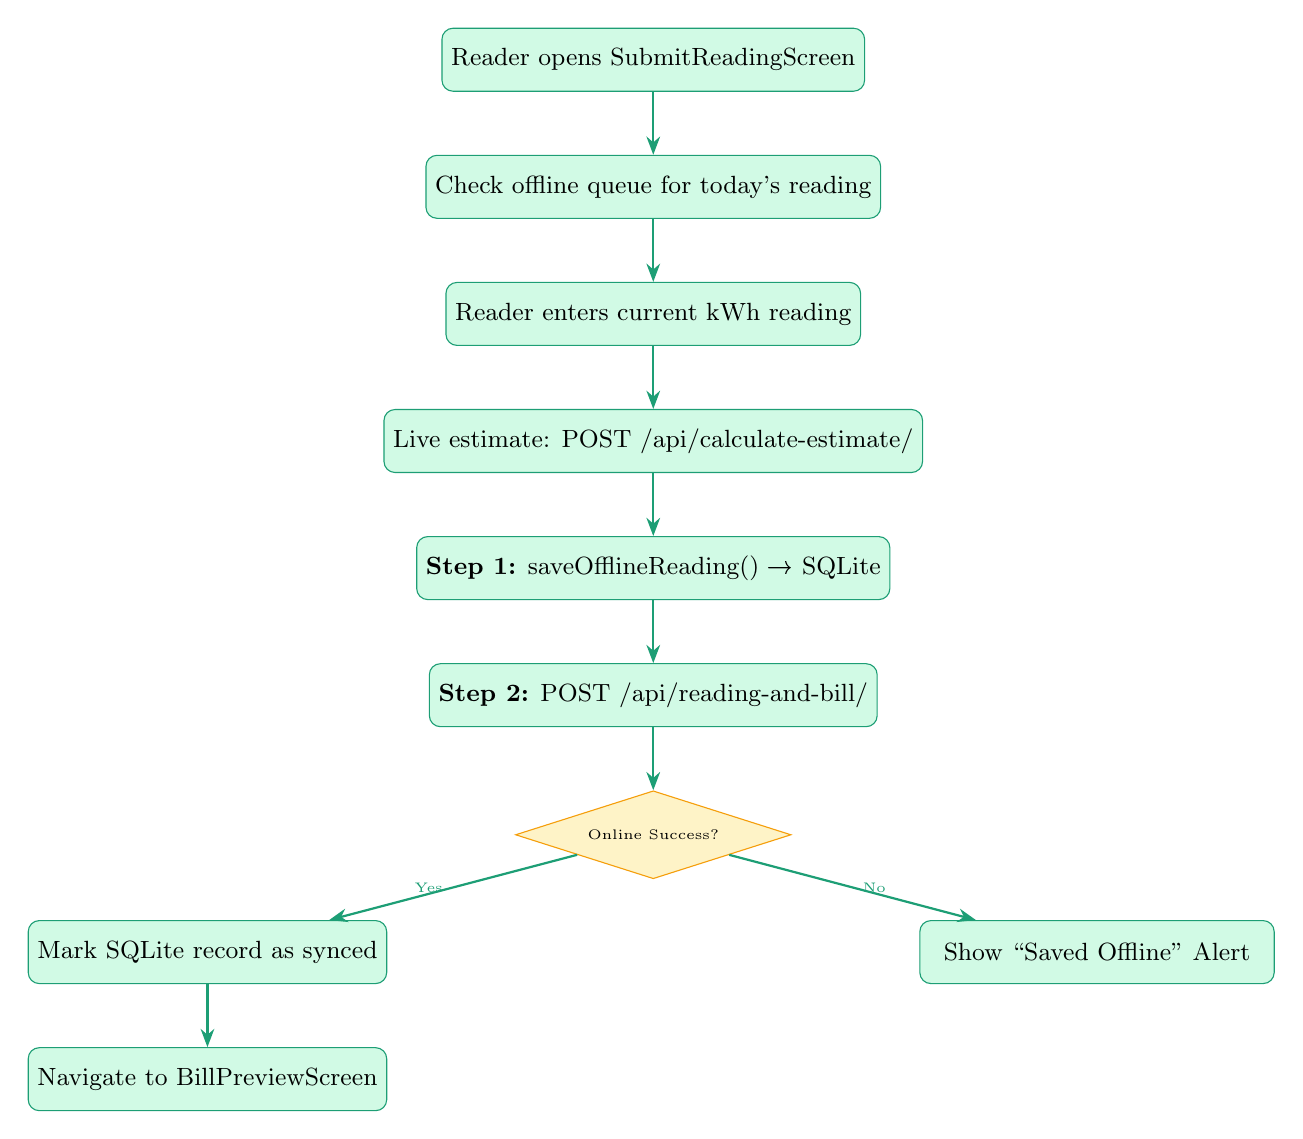
\begin{tikzpicture}[
    node distance=0.8cm and 0.5cm,
    process/.style={rectangle, rounded corners=4pt, minimum width=4.5cm, minimum height=0.8cm,
                    text centered, font=\small, fill=lightGreen, draw=primaryGreen},
    decision/.style={diamond, aspect=2.5, minimum width=3.5cm, minimum height=0.8cm,
                     text centered, font=\tiny, fill=warningBg, draw=accentAmber},
    storage/.style={rectangle, minimum width=4.5cm, minimum height=0.7cm,
                    text centered, font=\small, fill=codeGray, draw=borderColor},
    arrow/.style={-Stealth, thick, color=primaryGreen}
]

\node[process] (open) {Reader opens SubmitReadingScreen};
\node[process, below=of open] (check) {Check offline queue for today's reading};
\node[process, below=of check] (type) {Reader enters current kWh reading};
\node[process, below=of type] (estimate) {Live estimate: POST /api/calculate-estimate/};
\node[process, below=of estimate] (save_local) {\textbf{Step 1:} saveOfflineReading() → SQLite};
\node[process, below=of save_local] (try_online) {\textbf{Step 2:} POST /api/reading-and-bill/};
\node[decision, below=of try_online] (online_ok) {Online Success?};
\node[process, below left=of online_ok, xshift=-2cm] (mark_synced) {Mark SQLite record as synced};
\node[process, below=of mark_synced] (bill_preview) {Navigate to BillPreviewScreen};
\node[process, below right=of online_ok, xshift=2cm] (alert) {Show ``Saved Offline'' Alert};

\draw[arrow] (open) -- (check);
\draw[arrow] (check) -- (type);
\draw[arrow] (type) -- (estimate);
\draw[arrow] (estimate) -- (save_local);
\draw[arrow] (save_local) -- (try_online);
\draw[arrow] (try_online) -- (online_ok);
\draw[arrow] (online_ok) -- node[left, font=\tiny]{Yes} (mark_synced);
\draw[arrow] (mark_synced) -- (bill_preview);
\draw[arrow] (online_ok) -- node[right, font=\tiny]{No} (alert);

\end{tikzpicture}
\caption{Meter Reader — Reading Submission Flow}
\end{figure}

\section{Bill Finalization Flow}

\begin{figure}[H]
\centering
\begin{tikzpicture}[
    node distance=0.7cm,
    step/.style={rectangle, rounded corners=3pt, minimum width=9cm, minimum height=0.75cm,
                 text centered, font=\small, fill=lightBlue, draw=deepBlue},
    arrow/.style={-Stealth, thick, color=deepBlue}
]

\node[step] (s1) {1. Receive reading + consumer\_id from API};
\node[step, below=of s1] (s2) {2. Resolve active meter via ConsumerMeterAssignment};
\node[step, below=of s2] (s3) {3. validate\_reading(): chronology, duplicate, 20-day interval};
\node[step, below=of s3] (s4) {4. Create MeterReading record (units\_consumed = current − prev)};
\node[step, below=of s4] (s5) {5. Create Bill record (status = draft, is\_locked = False)};
\node[step, below=of s5] (s6) {6. calculate\_bill(): apply BillingSettings tariff};
\node[step, below=of s6] (s7) {7. Populate immutable snapshot fields};
\node[step, below=of s7] (s8) {8. Lock: is\_locked = True, status = issued};
\node[step, below=of s8] (s9) {9. Write AuditLog entry};
\node[step, below=of s9] (s10) {10. Return bill details to caller};

\draw[arrow] (s1) -- (s2);
\draw[arrow] (s2) -- (s3);
\draw[arrow] (s3) -- (s4);
\draw[arrow] (s4) -- (s5);
\draw[arrow] (s5) -- (s6);
\draw[arrow] (s6) -- (s7);
\draw[arrow] (s7) -- (s8);
\draw[arrow] (s8) -- (s9);
\draw[arrow] (s9) -- (s10);

\end{tikzpicture}
\caption{BillingService.generate\_final\_bill() — Processing Steps}
\end{figure}

% ============================================================
\chapter{Rebuilding the System: Developer Guide}
% ============================================================

\section{Prerequisites}

\begin{featurelist}
    \item Python 3.11+ and pip
    \item Node.js 18+ and npm/bun
    \item PostgreSQL 14+ (or use SQLite for development)
    \item Expo CLI (\texttt{npm install -g expo-cli})
    \item Git
\end{featurelist}

\section{Repository Structure}

\begin{lstlisting}[language=bash]
eMeter.web/
├── electricity_system/     # Django backend
│   ├── electricity_system/ # Django project settings
│   │   ├── settings.py
│   │   ├── urls.py
│   │   └── authentication.py
│   └── billing/           # Core application
│       ├── models.py       # All database models
│       ├── views.py        # All API views (2700+ lines)
│       ├── services.py     # BillingService (calculation engine)
│       ├── pdf_generator.py# ReportLab PDF generation
│       ├── permissions.py  # DRF permission classes
│       ├── urls.py         # URL routing
│       ├── admin.py        # Django admin registration
│       └── forms.py        # Django forms
├── energy-hub-ui/          # React + Vite Web SPA
│   └── src/
│       ├── pages/          # Route-level components
│       ├── components/     # Reusable UI components
│       ├── contexts/       # React context (Auth, Search)
│       ├── hooks/          # Custom hooks
│       └── lib/            # API client (axios)
└── eMeterApp/              # React Native Mobile App
    └── src/
        ├── screens/        # All screen components
        ├── services/       # api.js, offlineStorage.js, sqliteDb.js
        ├── context/        # Auth, Theme contexts
        ├── navigation/     # React Navigation setup
        ├── components/     # Reusable mobile components
        └── theme/          # Color themes
\end{lstlisting}

\section{Key Design Decisions to Understand Before Rebuilding}

\begin{enumerate}[leftmargin=1.8em, itemsep=6pt]
    \item \textbf{Single AUTH\_USER\_MODEL:} Always use \texttt{get\_user\_model()} or \texttt{settings.AUTH\_USER\_MODEL}. Never import \texttt{django.contrib.auth.models.User} directly.
    
    \item \textbf{Dual Auth Strategy:} Web clients use session cookies; mobile clients use Token Auth. Both authenticate at the same \texttt{/api/login/} endpoint.
    
    \item \textbf{Offline-First Mobile:} Every reading is saved to SQLite before attempting online submission. The online path is an enhancement, not a requirement.
    
    \item \textbf{Bill Immutability:} Once \texttt{is\_locked = True}, financial fields are frozen. Snapshots preserve the billing state at the moment of finalization for legal compliance.
    
    \item \textbf{Meter-Aware Readings:} All reading validation is per-meter, not per-consumer. A consumer may have multiple meters over time (via \texttt{ConsumerMeterAssignment}).
    
    \item \textbf{BillingSettings Singleton:} The tariff is stored in a single database row (id=1). Access always via \texttt{BillingSettings.get\_settings()} which has a safe fallback if DB is unavailable.
    
    \item \textbf{Consumption Anomaly:} After every reading, a background check computes 3-month rolling average. If new reading is 200\%+ above average, an admin notification is created.
    
    \item \textbf{SQLite Migration System:} The mobile app's SQLite schema uses a custom migration runner (based on \texttt{PRAGMA user\_version}) to upgrade existing users' local databases without losing data.
\end{enumerate}

% ─── Bibliography / References ──────────────────────────────
\chapter*{Appendix: Bill Calculation Example}
\addcontentsline{toc}{chapter}{Appendix: Bill Calculation Example}

\section*{Sample Calculation}

Given: Consumer with \textbf{load = 2 kW}, \textbf{analog meter}, \textbf{200 units consumed}

\vspace{0.5em}
Using current \texttt{BillingSettings} defaults:
\[
\text{rate\_per\_unit} = \text{Rs.}\ 8.56 \quad
\text{fixed\_charge\_per\_kw} = \text{Rs.}\ 400 \quad
\text{duty} = 7.5\% \quad
\text{phase\_1\_rent} = \text{Rs.}\ 10
\]

\begin{align*}
\text{Energy Charges} &= 200 \times 8.56 = \text{Rs.}\ 1712.00 \\
\text{Fixed Charges} &= 2 \times 400 = \text{Rs.}\ 800.00 \\
\text{Duty Charge} &= (1712 + 800) \times 0.075 = \text{Rs.}\ 188.40 \\
\text{Meter Rent} &= \text{Rs.}\ 10.00 \\
\text{Regulatory Surcharge} &= \text{Rs.}\ 0.00 \\
\text{Arrears} &= \text{Rs.}\ 0.00 \\
\text{Late Payment} &= \text{Rs.}\ 0.00 \\
\midrule
\textbf{Total Payable} &= \mathbf{1712 + 800 + 188.40 + 10 = \text{Rs.}\ 2711}
\end{align*}

\textit{Total is rounded to the nearest rupee (as per \texttt{round(..., 0)} in BillingService).}

\vspace{2em}
\hrule
\vspace{1em}

\begin{center}
\textit{End of eMeter AMU Actor \& Module Documentation}\\[0.3cm]
{\small Generated from source analysis of \texttt{anas36427/eMeter} — July 2026}
\end{center}

\end{document}
